
\section {Overview}
\label{sec-overview}

In this section, we give an informal overview of how an analyst would
use the framework to incrementally construct and analyze a model of a
system. We use an example from the web application domain to
illustrate our approach.

\paragraph{\textbf{Building an Initial Model}} Let us assume that the
director of the \textit{New York Times}, a well-known news
organization, wishes to design a \textit{paywall} system for its
online web site. A paywall system is used to limit readers to a set
number of free articles over a time period, requiring them to signup
for a paid subscription once they reach the limit. \suppress{At the
  same time, for optimal user experience, new users should not be
  required to create an account to start reading the articles.} One
desirable property of this paywall system is that \textit{readers who
  have already exceeded the limit should not be able to access an
  article}.

Alice, the chief web designer of the New York Times, devises a simple
design of the paywall system, as shown in
Figure~\ref{fig-nytimes}(a). There are three basic participants in this
design: the \textsf{NYTimes} server, which stores and serves articles,
\textsf{Reader}, an end-user who wishes to access an article, and
\textsf{Client}, which mediates the transfer of articles between
\textsf{NYTimes} and \textsf{Reader}. When \textsf{Reader} selects a
link to an article, \textsf{Client} forwards the request for the
article to the \textsf{NYTimes} server, sending along a counter
(\textsf{currCounter}) that represents the number of articles
\textsf{Reader} has accessed so far. \textsf{NYTimes} accepts a
 \textsf{GetPage} request from \textsf{Client} only if
\textsf{currCounter} is less than the limit. Once processing the
request, \textsf{NYTimes} then sends back a page that contains the
requested article, along with an increment of the original counter
(\textsf{newCounter}).

\begin{figure}[!t]
\centering
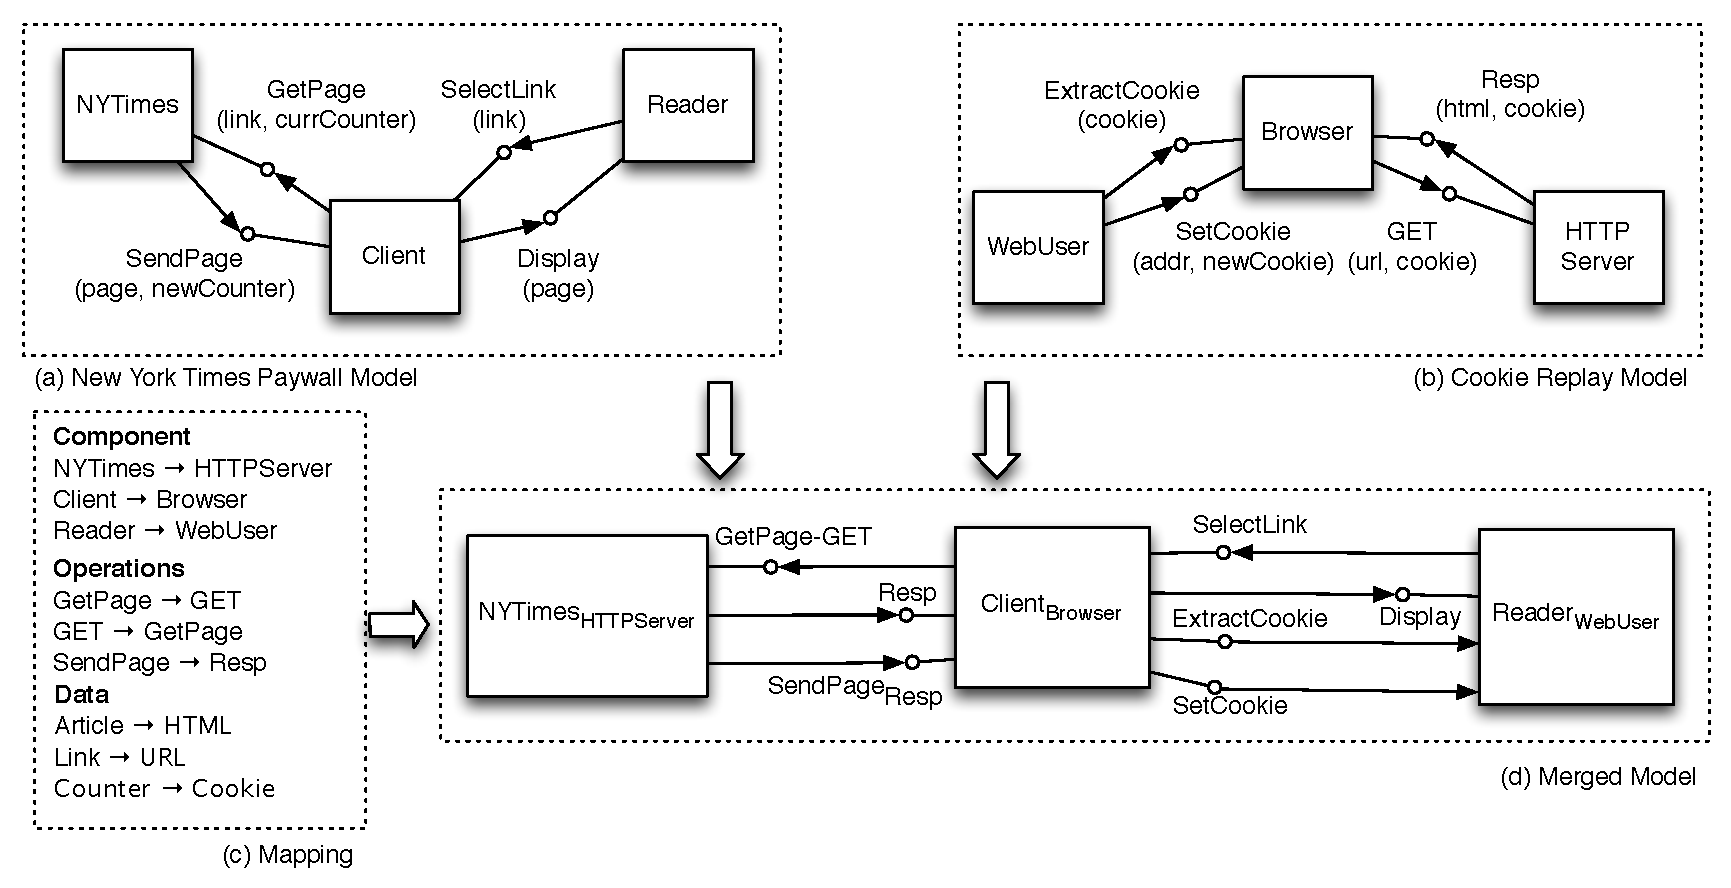
\includegraphics[width=1.0\textwidth]{diagrams/nytimes}
\caption{Models of (a) the New York Times paywall system and (b) a
  cookie replay attack, and (d) the result of merging the two models
  according to the mapping in (c). In each diagram, a box represents a
  component, and a directed edge from one component \textsf{A} to a
  port of another component \textsf{B} with label \textsf{O}
  represents \textsf{A}'s invocation of operation \textsf{O} that is
  exported by \textsf{B}. Each operation may require one or more
  arguments, listed inside brackets; for brevity, argument lists are
  omitted in (d).}
\label{fig-nytimes}
\end{figure}

Note that the model in Figure~\ref{fig-nytimes}(a) describes the system
interactions in terms of web API operations. This level of abstraction
is suitable for the designer to capture the essential functionality of
the system; it omits low-level details that are irrelevant to the
paywall workflow, such as what kind of devices various participants
are deployed on, how various API operations are implemented, or the
type of data structure that is used to represent counters and pages.

To ensure that the design is satisfactory, Alice decides to run the
model in Figure~\ref{fig-nytimes}(a) through an analysis engine that
exhaustively explores the behavior of the model. As expected, the
engine concludes that the system satisfies the property by preventing
the reader from accessing an article beyond the limit.

\paragraph{\textbf{Elaborating the System Model}} Being satisfied with the
initial design, Alice moves onto exploring lower-level design
choices for the system. She decides that \textsf{NYTimes} will run on
top of an HTTP server, with \textsf{GetPage} implemented as a
standard HTTP GET operation. Similarly, she
designates \textsf{Client} to run on top of a standard web browser,
and the access counter to be stored as a cookie inside the browser.

Alice decides to explore the potential implications of these design
decisions on the security of the system using our framework. \fix{Let
  us assume that the repository is already populated with models that
  describe different types of attacks that are applicable to web-based
  systems.}{She searches an existing repository of common security
  vulnerability models for web-based systems, finds a model of the
  \textit{cookie replay vulnerability}, and decides to check whether
  her system is susceptible to it}.

The cookie replay vulnerability involves a malicious user obtaining a
cookie and repeating its transmission to a server.  In
Figure~\ref{fig-nytimes}(b), \textsf{Browser} communicates to
\textsf{HTTPServer} by sending \textsf{GET} requests and receiving
responses (\textsf{Resp}) in return. In addition, a potentially
malicious browser user (named \textsf{WebUser}) interacts with
\textsf{Browser} by extracting a cookie from it
(\textsf{ExtractCookie}), or overwriting an existing cookie at a
particular address (\textsf{SetCookie}); this allows \textsf{WebUser}
to manipulate \textsf{Browser} into sending a request with a fixed
cookie value.

A next step for Alice would be to extend the original paywall model
with new details from the cookie replay model, and re-run the analysis
to see whether the elaborated model still satisfies the desired
property. However, the two models, as in their current form, are not
readily amenable to composition due to an \textit{abstraction
  mismatch}. These models describe the system at different layers of
abstraction, using two distinct sets of vocabulary terms to describe
components, operations, and data elements. They serve as \textit{partial}
descriptions of a system, including only the details of the system
that are necessary to illustrate a typical workflow (as in the paywall
model) or the characteristics of a particular attack (in the replay
model). Thus, additional guidance is needed to identify relationships
between parts of the two models before they can be merged.

Our observation is that relationships between a pair of models
correspond to the designer's decisions about how different parts of
the system are to be realized. For example, based on Alice's decisions
about the implementation of the paywall system, \textsf{NYTimes} can
be treated as a kind of \textsf{HTTPServer} that performs a
specialized function of serving articles to its client. A similar kind
of relationship can be specified between a pair of operations (e.g.,
\textsf{GetPage} and \textsf{GET}) or data sets (e.g, \textsf{Link}
and \textsf{URL}). Alice specifies these relationships as a mapping in
Figure~\ref{fig-nytimes}(c). Then, given this mapping, our framework
produces a new model that combines the characteristics of the two
models, as shown in Figure~\ref{fig-nytimes}(d).

\paragraph{\textbf{Re-Analyzing the Model}}

Alice re-runs the analysis engine on the merged model to check
whether the elaborated system still satisfies the desired
property. This time, the analysis engine discovers a counterexample
that demonstrates how the system might allow the reader to access an
article beyond the limit. In this scenario, \textsf{Reader}, now
acting as a \textsf{WebUser}, extracts a
cookie that represents the access counter prior to reaching the
limit. Then, \textsf{Reader} simply overwrites the existing cookie
with the extracted once the limit is exceeded, and \textsf{NYTimes}
continues to serve \textsf{GetPage} requests from
\textsf{Client}~\footnote{The actual paywall system for the New York
  Times suffered this type of attack when it was first introduced in
  2008~\cite{nytimes-attack}.}. To prevent this type of attack, Alice
modifies the system such that when \textsf{NYTimes} sends back a
cookie, it generates and includes a unique token that cannot be
guessed by \textsf{Reader}, thereby rendering old cookies invalid.

\am{CHECK: can we say the following?}
\ek{Not sure; I still have a mapping from read to webuser.
was:It is important to note that, to merge her initial model with
  the cookie replay attack, Alice did not have to explicitly specify
  that the \textsf{Reader} should be mapped to
  \textsf{WebUser}.  In contrast, Alice only had to specify her
  architectural decision to implement the system on top of HTTP, which
  meant implementing \textsf{NYTimes::GetPage} as
  \textsf{HTTPServer::GET} and \textsf{Client::SendPage} as
  \textsf{Browser::Resp}.  The information about potential
  vulnerability of HTTP systems to cookie replay is inherently present
  in the repository model, and our system is able to take advantage of
  it.}

Note that the mapping that Alice has provided is \textit{reusable};
any other model in the repository that describes interaction between
\textsf{HTTPServer} and \textsf{Browser} can be automatically merged
with the current system model. She may repeat the whole process
through multiple iterations, elaborating the system model with further
details from other vulnerability models, and re-running the analysis
engine to discover more potential design flaws.

\am{General comments: (1) renaming suggestions: GetPage
  $\rightarrow$ GetArticle, SendPage $\rightarrow$ ReceiveArticle,
  Client $\rightarrow$ NYTClient, Resp $\rightarrow$ ReceiveResp}
